%preamble
\documentclass[letterpaper]{article}
\synctex=1

\usepackage{listings}
\lstset{
%language=Assembler
% breaklines=true
%frame=single,
%xleftmargin=-1pt
}
\usepackage{geometry}
\usepackage{array}
\usepackage{lipsum}

\usepackage{graphicx}
\usepackage{float}
\graphicspath{ {images/} }

\usepackage{float}
% \usepackage[hidelinks]{hyperref}
% \usepackage[linktoc=all,hidelinks]{hyperref}
% \usepackage{bookmark}
% \usepackage[section]{placeins}
%
% \newenvironment{changemargin}[2]{%
% \begin{list}{}{%
% \setlength{\topsep}{0pt}%
% \setlength{\leftmargin}{#1}%
% \setlength{\rightmargin}{#2}%
% \setlength{\listparindent}{\parindent}%
% \setlength{\itemindent}{\parindent}%
% \setlength{\parsep}{\parskip}%
% }%
% \item[]}{\end{list}}

% \usepackage{tabu}
% \usepackage{blindtext}
%actual document
\begin{document}

  %titlepage
  \begin{titlepage}
    \begin{center}

      \LARGE
      ECE 212 Lab - Introduction to Microprocessors

      Department of Electrical and Computer Engineering

      University of Alberta

      \vspace{2cm}

      Lab 2: Introduction to Addressing Modes

      \vspace{5cm}
      \Large

      \begin{tabular}{ | m{5cm} | m{5cm} | }
        \hline
        Student Name & Student \\
        \hline
        Arun Woosaree & XXXXXXX \\
        \hline
        Navras Kamal & 1505463 \\
        \hline
      \end{tabular}

    \end{center}
\end{titlepage}

%table of tableofcontents

\tableofcontents

% \vfill
\newpage

\section{Introduction}
\textbf{FROM THE FIRST LAB  R E P L A C E T H I S!}
  The purpose of this lab is to learn and test with the Assembly language in a
  hands on environment in order to solidify the concepts learned in class and to
  improve our skill in the language.  In addition, we will be learning how to
  handle the Netburner ColdFire boards directly, manipulating the contents of
  their memory and data structures.  Finally, we are going to learn how to work
  inside the Eclipse IDE environment and how to properly use the powerful tools
  that come alongside it.

  The code will be developed for the Netburner ColdFire Platform, which has some
  parameters that should be kept in mind throughout testing.  There are multiple
  Data and Address registers, and the memory is indexed by hexadecimal codes.
  The data and the stored locations can each be modified directly, values can be
  compared and the code can branch into different sections depending on the
  values of the CCR (Condition Code Register) bits, which store information
  about the outcome from the last comparison or valid operation, such as if a
  value is negative or zero.  These will be used to execute code conditionally.

  The lab will be split into two sections, each with a different goal but with
  similar implementations. For one part we will be taking in an ASCII value and
  if the character it represents is a character included in the symbols for
  hexadecimal numbers then that hexadecimal value is output, otherwise it
  returns an error.  For the second part an ASCII value is taken in, and if the
  character it represents is a letter in the English language (A-Z) then the
  ASCII code for the character in the opposite case is output.  Thus, valid
  uppercase English letters are converted to their lowercase equivalents in
  ASCII and vice versa.

  These experiments will introduce implementing high level programming practices
  of loops, if - then - else statements, using the Assembly language. More
  specifically, this will introduce the movement of memory and data to and from
  different parts of the Netburner chip, using techniques such as referencing
  memory addresses and copying data to local data registers.  The debugger tools
  of the IDE will be used to closely examine this movement and to analyze all
  changes to the data in order to solve issues in development as well as to test
  the code.  This is all building off the concepts explored in Lab 0.

  The computing science practice of Pair Programming was also introduced, where
  two people develop and test code in tandem.  The partners are divided into the
  Driver and the Navigator. In this structure the Driver is the one responsible
  for the physical typing of the code into the computer, and the Navigator
  reviews this code and clarifies the meaning of each passage in order to find
  bugs faster and to improve efficiency in testing.  The two partners should
  communicate constantly and switch in order to maximize the efficiency of this
  working model. This will not only decrease time needed for development but it
  will also improve the quality of code from each partner.


\section{Design}

\subsection{Part A: Different Addressing Modes}
For part A of this lab, we wrote code to add the contents of two arrays
stored at different memory locations, and the result is stored at another
specified memory location. This is done using three  different addressing modes.
In the first part, we use Register Indirect With Offset, in the second part, we
use Indexed Register Indirect, and in the third part, we use Postincrement
Register Indirect. All information is stored as a long word (32 bits). The
operational code is provided at memory location 0x2300000, which contains the
information for where to access the arrays in memory and where to store the sum.
For example, the number stored at 0x2300000 contains the size of the arrays. The
operational code is stored as follows:

    \begin{enumerate}
      \item 0x2300000 - Size of arrays
      \item 0x2300004 - Address of first array
      \item 0x2300008 - Address of second array
      \item 0x230000C - Address of where to store the sum with Register Indirect With Offset
      \item 0x2300010 - Address of where to store the sum with Indexed Register Indirect
      \item 0x2300014 - Address of where to store the sum with Postincrement Register Indirect
    \end{enumerate}

    \begin{figure}[h!]
      \centering
      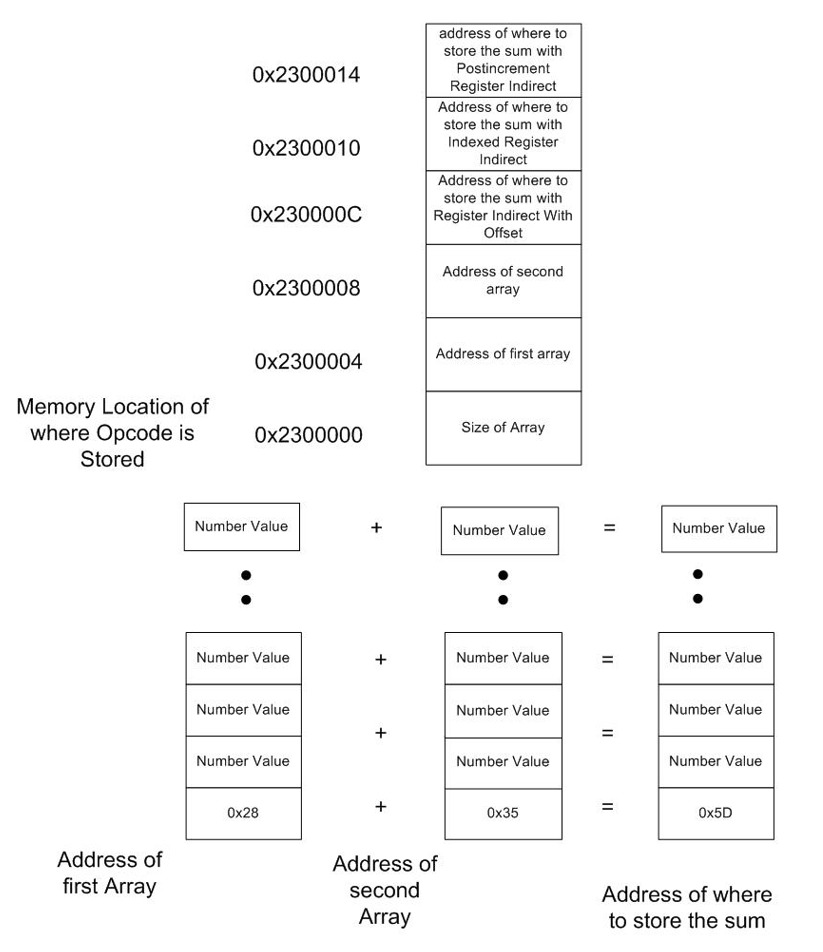
\includegraphics[width=.6\textwidth]{mema.jpg}
      \caption{An illustration of how the data is organized in part A}
    \end{figure}

    \noindent The \textit{SetZeros.s} and the \textit{DataStorage.s}
    files, which were provided, were used to initialize memory contents.

    \subsubsection{Part 1: Register Indirect With Offset}
    We chose address register a1 to store the contents at 0x230000C, which is
    where the address to output the sum is located. This was done by loading the
    effective address into a1, and moving the contents of the memory location
    stored at a1 into a1 itself. In a similar fashion, address register a2 was
    chosen to store the contents at 0x2300004, which stores the starting address
    of the first array to be added. Similarly, address register a3 was chosen to
    store the location of where the second array to be added starts, and that
    memory address is stored at 0x2300008. To add the first two numbers in the
    arrays, the contents of the memory location pointed to by a2 were moved into
    data register d3, and the contents of the memory location pointed to by a3
    were added to d3. The result in d3 was then stored at the memory location
    pointed to by a1. Next, these three lines of code were copy-pasted and
    modified to add offsets to the memory locations.  So, to add the next two
    numbers in each array, the contents of the memory location (4,\%a2) was
    moved to d3, the contents of the memory location (4,\%a3) was added to d3,
    and the result in d3 was moved to the memory location (4,\%a1). The same
    method was applied to add the third numbers in the arrays, but this time
    with an offset of 8.


    \subsubsection{Part 2: Indexed Register Indirect}
    The loading of the memory addresses in part 2 was done very similarly to part 1.
    Address registers a2 and a3 still contain the memory locations of where the
    first and second array begin. However, the contents at memory location
    0x2300010 was moved to a1, which is where the result is stored for this
    part. Data register d1 was chosen to store the amount by which we want to
    offset, and d2 was chosen to be our counter variable for a loop.
    Additionally, both these data registers were cleared. Inside the loop, the
    contents of the memory location stored by a2 were moved to d3, just like in
    part 1. Except this time, it was offset by the number in d1. So, on the
    first loop iteration, it would be displaced by 0. Similarly, the contents of
    the memory location pointed to by a3, displaced by the value at d1, is added
    to d3. The result stored in d3 is then moved to the memory location a1, also
    displaced by the number stored in d1. At the end of the loop, we increment
    the offset d1 by 4, and the counter is incrmented by 1. Then, we compare our
    counter to the size of the arrays, which is a value stored at 0x2300000, and
    if our counter is less than the size of the array, we continue the loop.


    \subsubsection{Part 3: Postincrement Register Indirect}
    Loading of the memory addresses in part 3 was also very similar to parts 1 and
    2. Address registers a2 and a3 are unchanged, but the  contents at memory
    location 0x2300014 was moved to address register a1, which is where the
    result is stored in this part. We chose data register d2 to be our counter
    variable, which was initially cleared with the value of 0. Just like for
    part 2, we have a loop, but this time there are no offsets. Instead, we move
    the contents of the memory location pointed to by a2 to d3, and
    postincrement a2. Similarly, the contents fo the memory location pointed to
    by a3 is moved to d3, and a3 is post incremented. At the end of the loop,
    the counter is incremented by 1, and if it is less than the size of the
    arrays (stored at 0x2300000), the loop continues.


    % \subsubsection{Part A Sample Calculations of Conversion}
    %     \textbf{from the last lab}
    %     input = `9' = 0x39\\
    %     0x39 - 0x30 = 0x9\\
    %     \\
    %     input = `E' = 0x45\\
    %     0x45 - 0x41 = 0x4\\
    %     0x4 + 0xA = 0xE\\
    %     \\
    %     input = `d' = 0x64\\
    %     0x64 - 0x61 = 0x3\\
    %     0x3 + 0xA = 0xD



  \subsection{Part B: Trapezoidal Rule}

    In part B of this lab,we write a program that calculates the area
    underneath a curve ($y=f(x)$), using the trapezoidal rule:
    $$ \int_a^b f(x) dx \approx \sum_{k=1}^{N} \frac{f(x_{k-1})+f(x_k)}{2}\Delta x_k$$
    The x and y data points for the curve are stored in arrays, at different
    memory addresses. For convenience, the distance between each X data point is either one
    or 2 units. Similar to part A, we have some operational code stored at 0x2300000, which contains the
    information for where to access the arrays in memory and where to store the output.
    The operational code is as follows:

    \begin{enumerate}
      \item 0x2300000 - Number of Data Points
      \item 0x2300004 - Address of where the X data points are stored
      \item 0x2300008 - Address of where the Y data points are stored
      \item 0x230000C - Address of temporary storage space
      \item 0x2300010 - Address of where to store the final output
    \end{enumerate}

    \begin{figure}[h!]
      \centering
      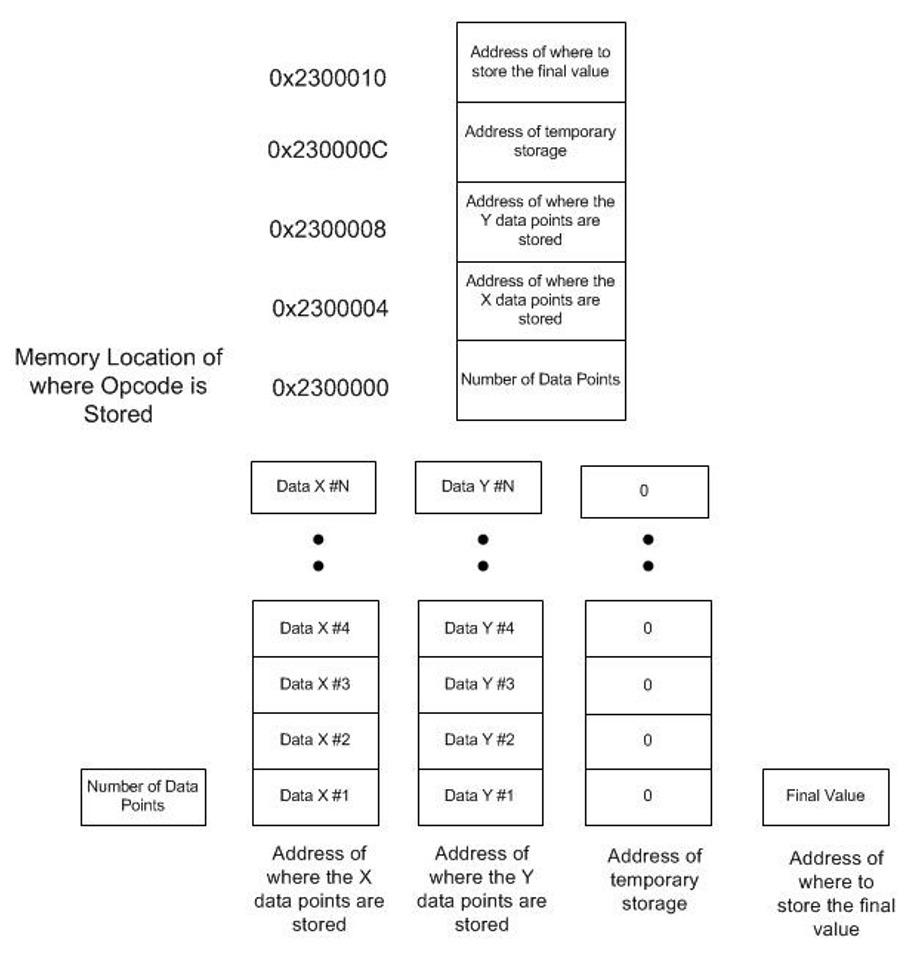
\includegraphics[width=0.6\textwidth]{memb.jpg}
      \caption{An illustration of how the data is organized in part B}
    \end{figure}

    In our initialization, we chose d0 to store the total number of data points,
    by moving the contents at 0x2300000 to d0, then subtracting 1 from d0 to
    avoid an off-by-one indexing error. a0 was chosen to store the address of
    the array with X data points, so the contents at 0x2300004 were moved to a0.
    Similarly, the contents at 0x2300010 were moved to a2, to store the address
    of the array with Y data points. Data register d1 was used as a counter, and
    d7 stores the total area. Both of these data registers were cleared with
    initial value 0. Initial data points $x_0$ and $y_0$ were stored in d2 and
    d3, respectively. Once our initialization is done, we enter a main loop,
    where we decided to do our checks for exiting the loop at the beginning. The
    loop exits if our counter (d0) is equal to the number of points (d1),
    otherwise the counter is incremented. In the loop, the contents of the
    memory address pointed to by a0 is moved to d4, and post incremented, so
    that d4 holds $x_k$. Similarly, the contents of the memory address pointed
    to by a1 is moved to d5, and post incremented, so that d5 holds $f(x_k)$. We
    get $f(x_{k-1})+f(x_k)$ by adding d5 to d3 and storing the result in d3.
    Then, $\Delta x$ is calculated by subtracting d4 from d2, storing the
    negation of that result in d2. If $\Delta x$ was 2, we multiplied d3, which
    was $f(x_{k-1})+f(x_k)$ by 2 and then added the result to d7. If $\Delta x$
    was not 2, we just added $f(x_{k-1})+f(x_k)$ to d7. At the end of the loop,
    $x_k$ and $f(x_k)$ from the current iteration are set to be $x_{k-1}$
    $f(x_{k-1})$ respectively, for the next iteration by moving the contents of
    d4 to d2 and also moving the contents of d5 to d3. When the loop terminates,
    we check if the number in d7 is odd by checking its least significant bit.
    If it is odd, we add one to it. Finally, the number in d7 is divided by 2
    using a right bit shift operation, and the result is moved into the memory
    location pointed to by a2, which is where the ourput should go. We check if
    the number in d7 is odd before dividing it by 2, so that our program would
    round the number up if we get a fraction, as per the assignment
    specifications.

%     \subsubsection{Part B Sample Calculations of Conversion}
%     \textbf{from the last lab}
%     input = `M' = 0x4D\\
%     0x4D + 0x20 = 0x6D\\
%     0x6D = 'm'\\
%     \\
%     input = `d' = 0x64\\
%     0x64 - 0x20 = 0x44\\
%     0x44 = 'D'


\section{Testing}
  \subsection{Part A}
    Initially, we visually tested our code by using the debugger in Eclipse IDE.
    While stepping through the code, we would check the values at relevant
    memory locations, and the data and address registers. Initially, for part 3,
    we had an error where the sum calculated in the output array was all zeros.
    However, we later discovered that while exiting our loop in part 2, we
    jumped to the end of the program, so part 3 would never run. When the bugs
    were ironed out, After we fixed this minor bug, we went on to the next phase
    of testing. Our code was tested using the provided \textit{Lab2aTest.s}
    file. More specifically, this program was moved into the project folder,
    downloaded to the ColdFire microcontroller, and the MTTTY serial monitor was
    loaded to monitor the expected output. Our code was further tested by
    replacing the `DataStorage.s' file with the other variants provided named:
    \textit{DataStorage1.s}, \textit{DataStorage2.s}, and
    \textit{DataStorage3.s}. Finally, our program, which produced the correct
    output, was verified by a lab TA, who further tested our code by modifying
    the DataStorage file and verifying the output.
    \begin{figure}[H]
      \centering
      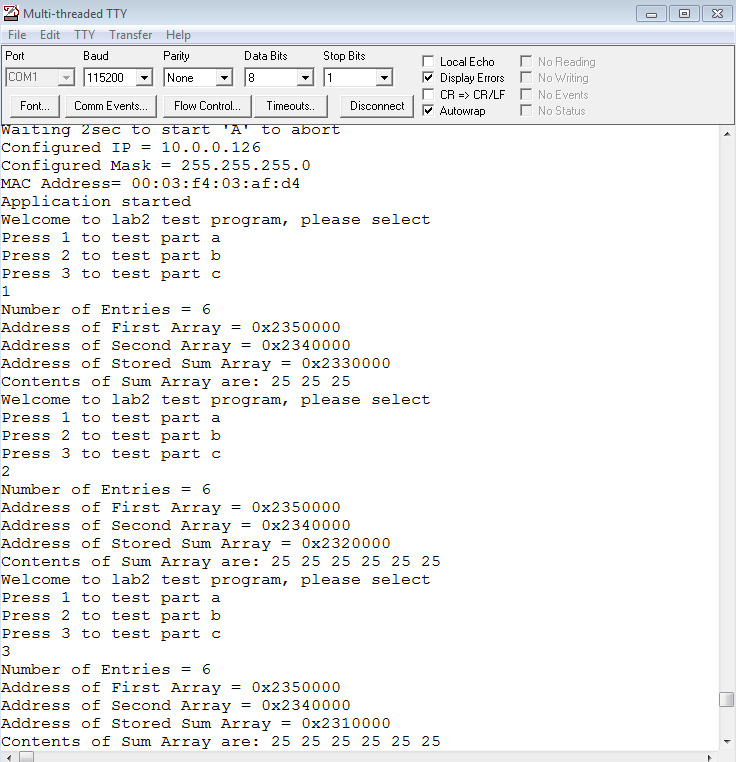
\includegraphics[width=.65\textwidth]{part1.jpg}
      \caption{MTTTY output when testing our Part A solution}
    \end{figure}

  \subsection{Part B}
    Although the parts were different, the procedure for testing our code for
    part B was similar to the process described above in Part A. We visually
    inspected our code in the Eclipse IDE, used the Eclipse debugger to step
    through our code, and monitored relevant memory addresses and registers. We
    initially got a huge number, above 63 million, which we correctly identified
    as an off-by-one indexing error. This problem was rectified by subtracting
    one from d0, which is what we used to store the total number of points. We
    also included some code towards the end which  would make sure our code
    rounds up as per the lab specifications if we got a fraction instead of a
    whole number when calculating the area (as verified by a lab TA). However,
    this code seemed to have no effect, since our program produced the correct
    output anyways. Our program still worked with this code, however as it was not
    fully tested we left it commented out in our submission. After review we have
    seen that there is a more elegant way to reach the same solution using bit tests
    but we have left it as it was at the time that it was reviewed by the TAs in lab.
    In any case, we used the provided files \textit{Lab2bTest.s}, and the
    \textit{Datastorage5.s} files to verify our solution by downloading the
    program to the ColdFire microcontroller, and monitoring the output in MTTTY.
    Finally, our solution was verified by a lab TA. As per the lab instructions,
    we used \textit{DataStorage5.s} and \textit{SetZeros5.s} files, although we
    did further test our program using \textit{DataStorage4.s} with a lab TA and
    found no issues.


    % \begin{figure}[H]
    %   \centering
    %   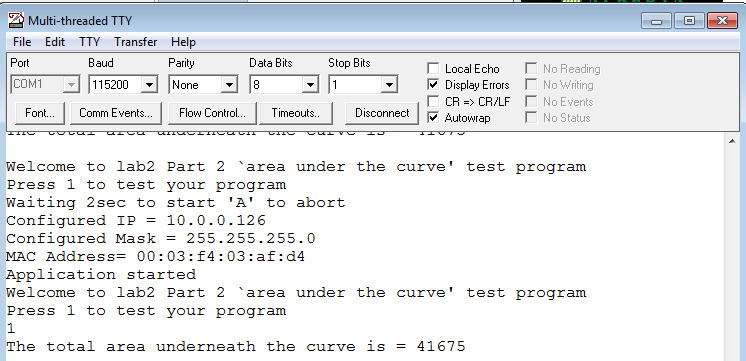
\includegraphics[width=0.6\textwidth]{part2ds4.jpg}
    %   \caption{MTTTY output when testing our Part B solution with \textit{Datastorage4.s}}
    % \end{figure}

    \begin{figure}[H]
      \centering
      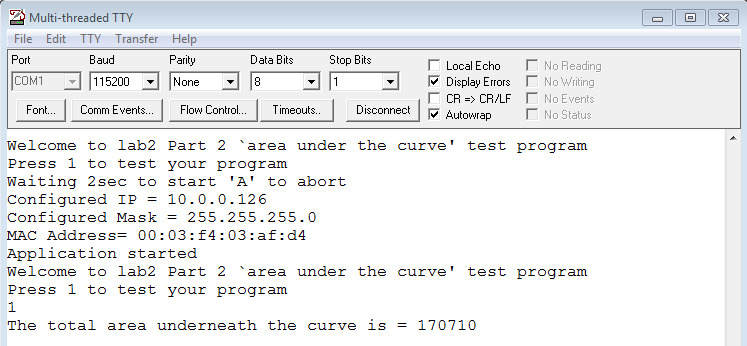
\includegraphics[width=0.9\textwidth]{part2ds5.jpg}
      \caption{MTTTY output when testing our Part B solution with \textit{DataStorage5.s}}
    \end{figure}

\section{Questions}
  \begin{enumerate}
    \item \textit{What are the advantages of using the different addressing modes covered in this lab?}
          % \textbf{A: }
          \begin{enumerate}
            \item Register Indirect With Offset
              \begin{enumerate}
                \item Great if you only plan on accessing one thing
                \item Doesn't modify the address register's value
                \item Can access any memory address you want relative to the value stored in the address register
              \end{enumerate}
            \item Indexed Register Indirect
            \begin{enumerate}
              \item Doesn't modify the address register's value
              \item You can offset in terms of a variable, so you have greater control over the offset
              \item Works well in loops
            \end{enumerate}
            \item Postincrement Register Indirect
            \begin{enumerate}
              \item You don't have to keep track of the offset, it automatically
                    increments the address register by the size of the data
                    you're working with
              \item Very useful for dealing with arrays
              \item Works nicely in loops
            \end{enumerate}
          \end{enumerate}

    \item \textit{If the differece between the X data points are not restricted to be either one
                  or two units, how would you modify your program to calculate the area? You do
                  not need to do this in your code.}\\
          \textbf{A: }
          Instead of hard coding two scenarios where $\Delta x$ is either 1 or 2,
          we could just divide $f(x_{k-1})+f(x_k)$ by 2 with a bit shift operation
          to the right by one, and then use the \textit{muls.l} instruction
          to multiply the result by $\Delta x$ to match the equation for the trapezoidal rule.
    \item \textit{From the data points, what is the function (y=f(x))? What is the percent error between the
                  theoretical calculated area and the one obtain in your program?}\\
          % \textbf{A: }
          \\From the data points, we can tell the function is $y=x^2$.\\
          The value obtained in our program was \textbf{170710}.\\
          The actual value should be:\\
          $$\int_0^{80} x^2 dx = \frac{x^3}{3}\Big|_0^{80} = \frac{80^3}{3} = \frac{512000}{3}= \textbf{170666.666...} $$
          Therefore, the percent error is:
          $$\frac{|\frac{512000}{3}-170710|}{\frac{512000}{3}}\times 100 = \frac{13}{512}\% = \textbf{0.025390625\%}$$

  \end{enumerate}

\section{Conclusion}
\textbf{from the last lab}
This lab demonstrated how to perform operations and modify data while
moving it around using the Assembly language for the ColdFire architechture. In
addition, the lab improved our understanding of the debugger software, a very
powerful tool in the development of this kind of code.  The main issue we found
was related to the hardware itself, as there was some instances where the code
did not execute properly and the board itself needed to be reset.  The other
issue we faced was mostly around getting used to the software and the workflow
in the Eclipse IDE and the debugger.  Once we understood the ways to use the
tools we found our workflow sped up considerably, as we were able to check step
by step and find bugs at the source.  The last issue we had was with the syntax
of the code, but that was solved quickly by reading over documentation and with
the help of the TAs.  Overall the lab went smoothly and has indeed succeeded at
the goals of improving our familiarity and skill with the Netburner ColdFire
system, Assembly code and Pair Programming practices.

\newpage
\section{Appendix}
  %\textwidth=600pt
  \subsection{Part A Assembler Code}
    % \begin{changemargin}{-2cm}{-2cm}
    \lstinputlisting{code/Lab2a.s}
  % \end{changemargin}
\newpage


  \subsection{Part A Flowchart Diagrams}

  \subsubsection{Part 1: Register Indirect With Offset}
  \vspace{2cm}
  \noindent\makebox[\textwidth]{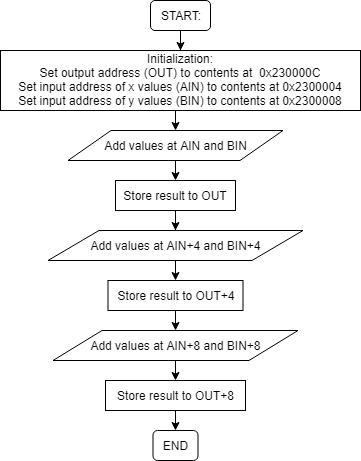
\includegraphics[width=\paperwidth,height=\paperheight,keepaspectratio]{partaflowchart1.jpg}}
\newpage

  \subsubsection{Part 2: Indexed Register Indirect}
  \vspace{2cm}
  \noindent\makebox[\textwidth]{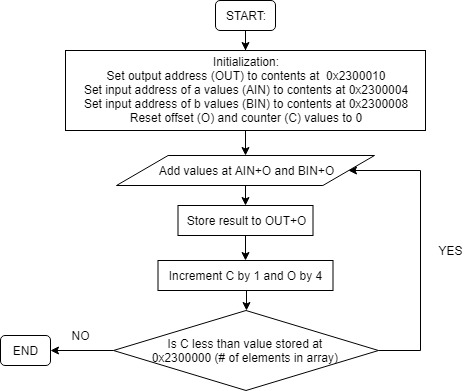
\includegraphics[width=\paperwidth,height=\paperheight,keepaspectratio]{partaflowchart2.jpg}}
\newpage

  \subsubsection{Part 3: Postincrement Register Indirect}
  \vspace{2cm}
  \noindent\makebox[\textwidth]{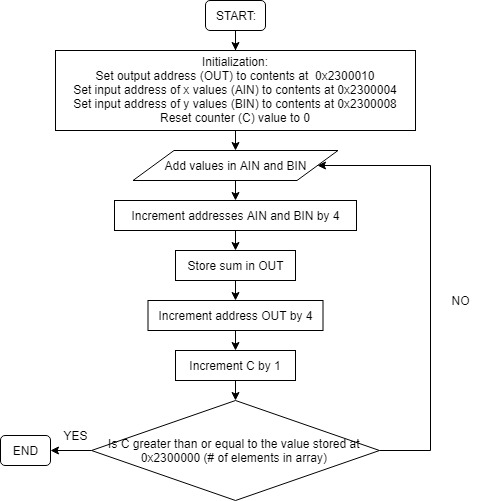
\includegraphics[width=\paperwidth,height=\paperheight,keepaspectratio]{partaflowchart3.jpg}}
\newpage


  \subsection{Part B Assembler Code}
    \lstinputlisting{code/Lab2b.s}
\newpage

  \subsection{Part B Flowchart Diagram}
  \vspace{2cm}
    \noindent\makebox[\textwidth]{
\includegraphics[width=\paperwidth,height=\paperheight,keepaspectratio]{partbflowchart.jpg}}
\newpage
% \@
% % \pagenumbering{gobble}
% % \addcontentsline{toc}{section}{Marking Sheet}
% % \section{Marking Sheet}
% % \clearpage
% \addtocounter{section}{1}
% % \addcontentsline{toc}{section}{Marking Sheet}
% \addcontentsline{toc}{section}{\protect\numberline{\thesection} Marking Sheet}

\section{Marking Sheet}
\end{document}
